\documentclass[12pt]{beamer}
\usepackage{CJKutf8} 
\usepackage{graphicx}
\usepackage{hyperref}
\usepackage{cite}
\usepackage[normalem]{ulem} % use normalem to protect \emph

\usetheme{Boadilla}
\usecolortheme{beaver}

\renewcommand{\[}{\begin{equation*} \begin{aligned}} % substitute `\[`, `\]` for aligned equations
	\renewcommand{\]}{\end{aligned} \end{equation*}}

\title[WeChat Red Envelope Modeling]{Algorithmic Mechanism Modeling of WeChat Red Envelope Game}
\author{Guanzhou Hu}
\institute[ShanghaiTech]{School of Information Science and Technology \\ShanghaiTech University}
\date{January 18, 2018}
\begin{document}

\begin{frame}
	\titlepage
\end{frame}

\begin{frame}{Abstract}
	\ \ This presentation focuses on the analysis and simulation of stochastic algorithmic mechcanism behind WeChat Red Envelopes. The whole process from raw data analysis, model hytheses testing to algorithm simulation will be included. A good approximation of WeChat Red Envelope algorithm will finally get put forward.
\end{frame}

\begin{frame}
  \frametitle{Outline}
  \tableofcontents
\end{frame}

\AtBeginSection[]
{
\begin{frame}{Outline} \tableofcontents[currentsection]
	\end{frame}
}

\section{Introduction}

\begin{frame}{Problem Description}
	\ \ WeChat Red Envelope is a popular social game based on WeChat Platform. It gains popularity mainly from its randomness. \\[6pt]
	\textbf{Game Process}: \begin{enumerate}
		\item The sender plugs in a certain amount of money $m$ into a virtual red envelope, sets the restriction of envelope size $n$ - the number of people that can open this envelope, and sends it into a chat group.
		\item Members in the group can open this envelope and grab a random amount of money, as long as the limitation of number of people is not exceeded.
	\end{enumerate}
\end{frame}

\section{Data Collecting and Analysis}

\begin{frame}{Data Analysis}
	\begin{itemize}
		\item Dataset is generated within two chat groups of $36$ members.
		\item Red envelope size is fixed as 
			\[
				\text{[Amount $m = 10$ Yuan / Number of people $n = 10$]}
			\]
			during the analysis stage, in the purpose of regulation and normalization of data.
		\item Overall $202$ pieces of valid data are collected.
	\end{itemize}
\end{frame}

\begin{frame}{Data Analysis}
	\begin{definition}
		\ \ Denote the order of snatching as position $0, 1, \dots , 9$. Let $A_i$ be the amount of money that is grabbed by position $i$, $i \in \{0, 1, \dots , 9\}$
	\end{definition}
	\vspace{6pt}
	Therefore $\sum_{i=0}^9 A_i = 10$ for each envelope.
\end{frame}

\begin{frame}{Mean and Variance at Positions}
	\begin{itemize}
		\item The \textit{mean} of $A_i$ shows great uniformity among different positions.
		\item \textit{Variance} at latter positions are generally larger, and reveals a jump at position $8$.
	\end{itemize}
	\centering
	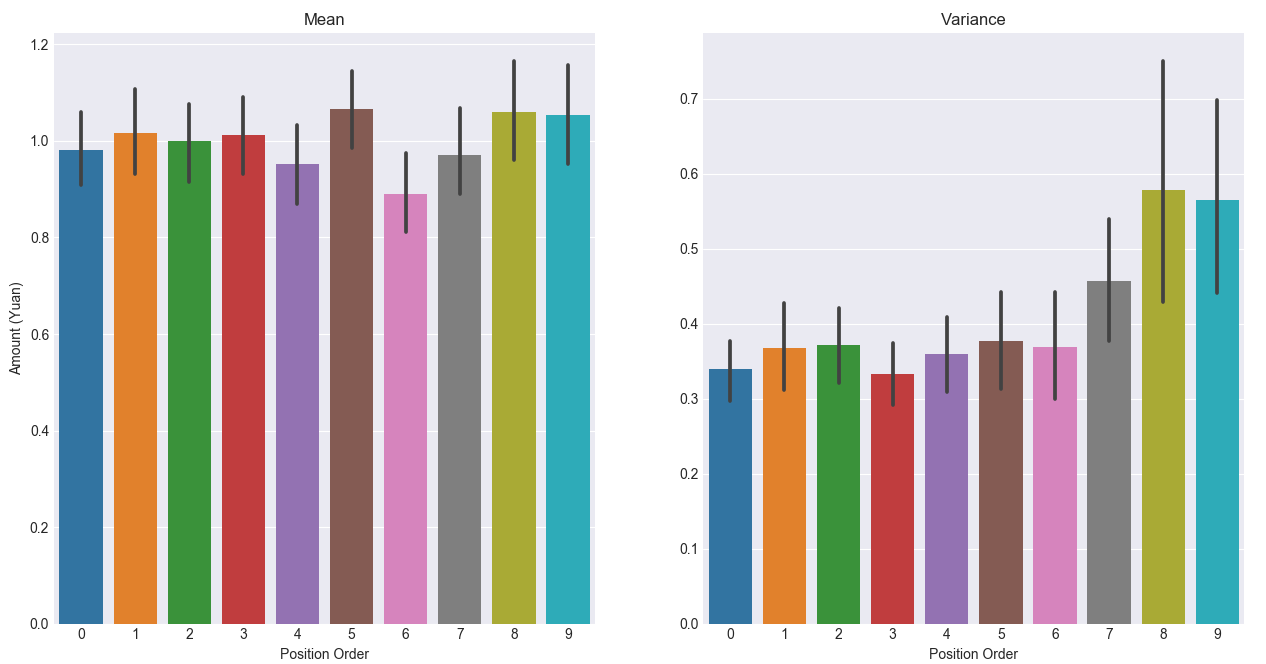
\includegraphics[scale=0.3]{data1.png}
\end{frame}

\begin{frame}{Distribution at Positions}
	\ \ $A_i$ approximately follows a Uniform distribution for smaller order positions, and a truncated Normal distribution for latter positions.
	\vspace{16pt}
	\centering
	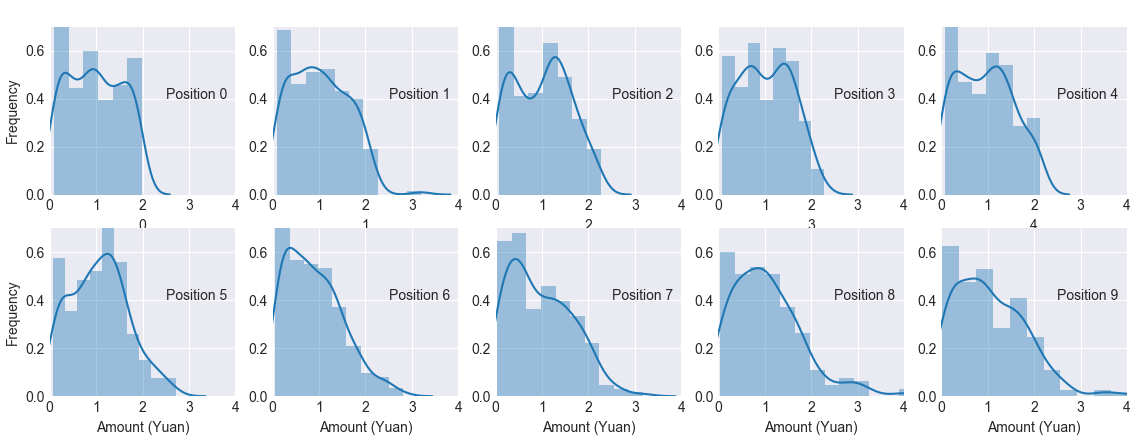
\includegraphics[scale=0.4]{data2.png}
\end{frame}

\begin{frame}{Max and Min Amount in Envelopes}
	\begin{itemize}
		\item The Maximum amount of money in each red envelope is generally larger than $1.5$ Yuan, and smaller than $2.0$ Yuan, except for some outstanding peaks which reach the largest value of $4.21$ Yuan.
		\item The Minimum amount is generally smaller than $0.5$ Yuan, and touches the smallest possible value of $0.01$ Yuan in some envelopes.
	\end{itemize}
	\centering
	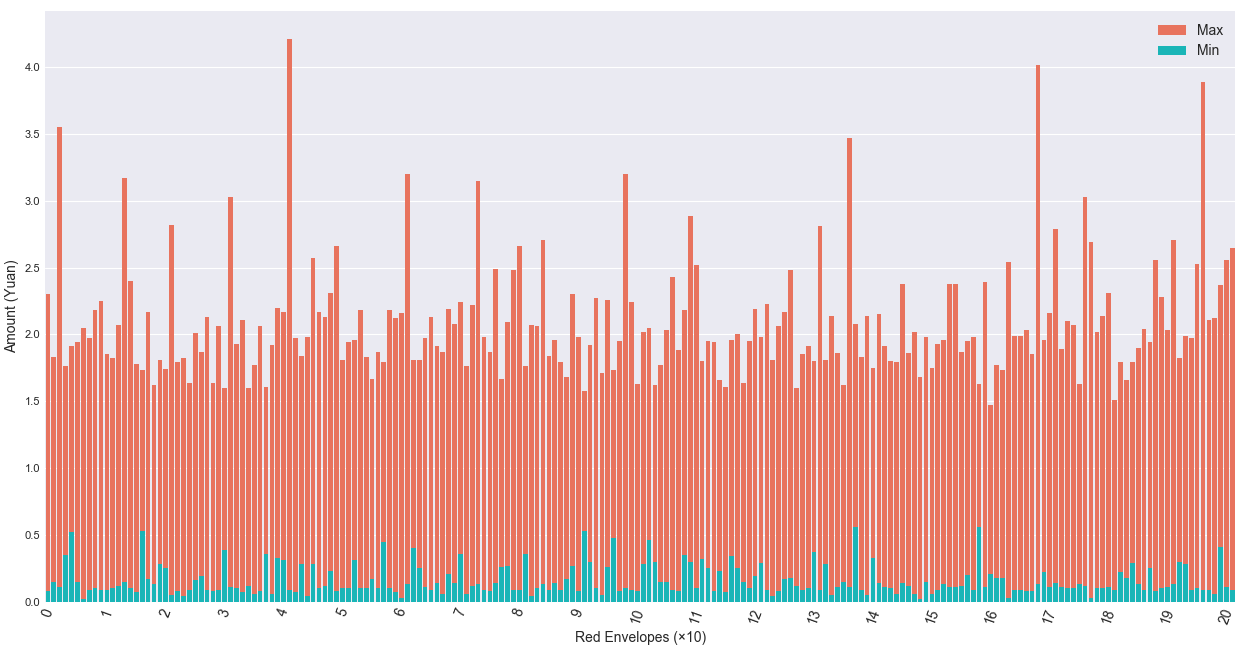
\includegraphics[scale=0.25]{data3.png}
\end{frame}

\begin{frame}{Data Features}
	\begin{enumerate}
		\item Each position has a \textbf{generally stable mean} around $m/n = 1$.
		\item \textbf{Variance is slightly increasing, and shows a large jump at the penultimate position.}
		\item Smaller order positions, \textbf{especially the first position, reveal an Uniform distribution}, meanwhile \textbf{the latter positions show a truncated Normal distribution.}
		\item The Min amount of money basically ranges from $0.01$ Yuan to $0.5$ Yuan, and has the possibility of touching the very bottom.
		\item The Max amount of money basically ranges from $1.5$ Yuan to $2.0$ Yuan, and has the possibility of reaching a respectively large value of over $4.0$ Yuan.
	\end{enumerate}
\end{frame}

\section{Model Hypotheses}

\begin{frame}{Model Hypotheses}
	\ \ Based on the five observations, the following two hypotheses of algorithm models are proposed and will be examined mathematically.
	\begin{itemize}
		\item \textit{Static-Uniform Model}
		\item \textit{Dynamic-Updating Model}
	\end{itemize}
\end{frame}

\begin{frame}{Static-Uniform Model}
	\ \ Suppose the allocation of money inside every red envelope is completely computed at the exact sending time. The envelope seen by chat group members is simply static, offline package of numbers. Every time the envelope is snatched, it returns a uniformly randomly chosen number inside the package.
\end{frame}

\begin{frame}{Static-Updating Model}
	\centering
	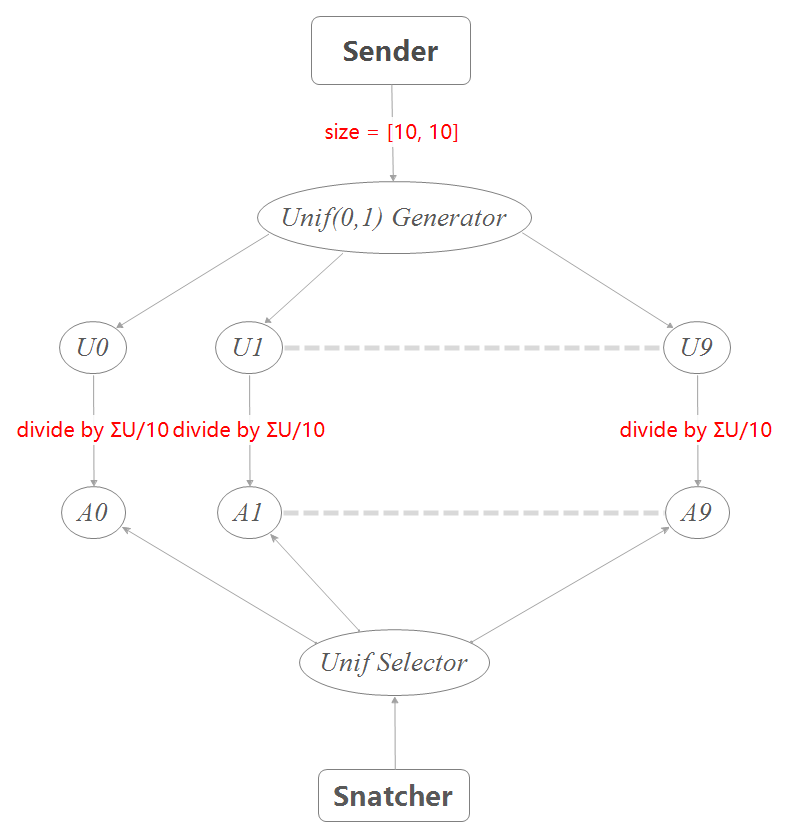
\includegraphics[scale=0.25]{model1.png}
\end{frame}

\begin{frame}{Static-Uniform Model}
	\textbf{Mathematical Verifications}:
	\begin{itemize}
		\item Expectation of $A_i$:
			\[
				E(A_i) = \frac{E(\sum_{j=0}^{9} A_j)}{10} = 1
			\]
			for all $i \in \{0, 1, \dots ,9\}$.
		\item Max and Min value in each envelope: Since $U_0, U_1, \dots , U_9 \sim$ Unif($0, 1$), the $j$th order statistics $U_{(j)} \sim$~Beta($j, 10-j+1$). Therefore,
			\[
				P(U_{min} \le 0.25) = P(U_{(1)} \le 0.25) \approx 0.947 \\
				P(U_{max} \ge 0.75) = P(U_{(10)} \ge 0.75) \approx 0.947
			\]
			which agrees with insight 4) and 5).
	\end{itemize}
\end{frame}

\begin{frame}{Dynamic-Updating Model}
	\ \ Suppose the amount of money snatched from the red envelope is generated dynamically at the time when a member opens it. Under this scenario, the amount of money $A_0 A_1, \dots ,A_9$ grabbed by different positions are dependant with each other. Therefore, every generating of $A_i$ is influenced by its position $i$ and the rest money $m_i'$. A significant restriction that might get neglected is that every person should at least grab $0.01$ Yuan, therefore when the algorithm reaches the stage $A_8$, it needs some adjustments to ensure $A_9 \ge 0.01$.
\end{frame}

\begin{frame}{Dynamic-Updating Model}
	\centering
	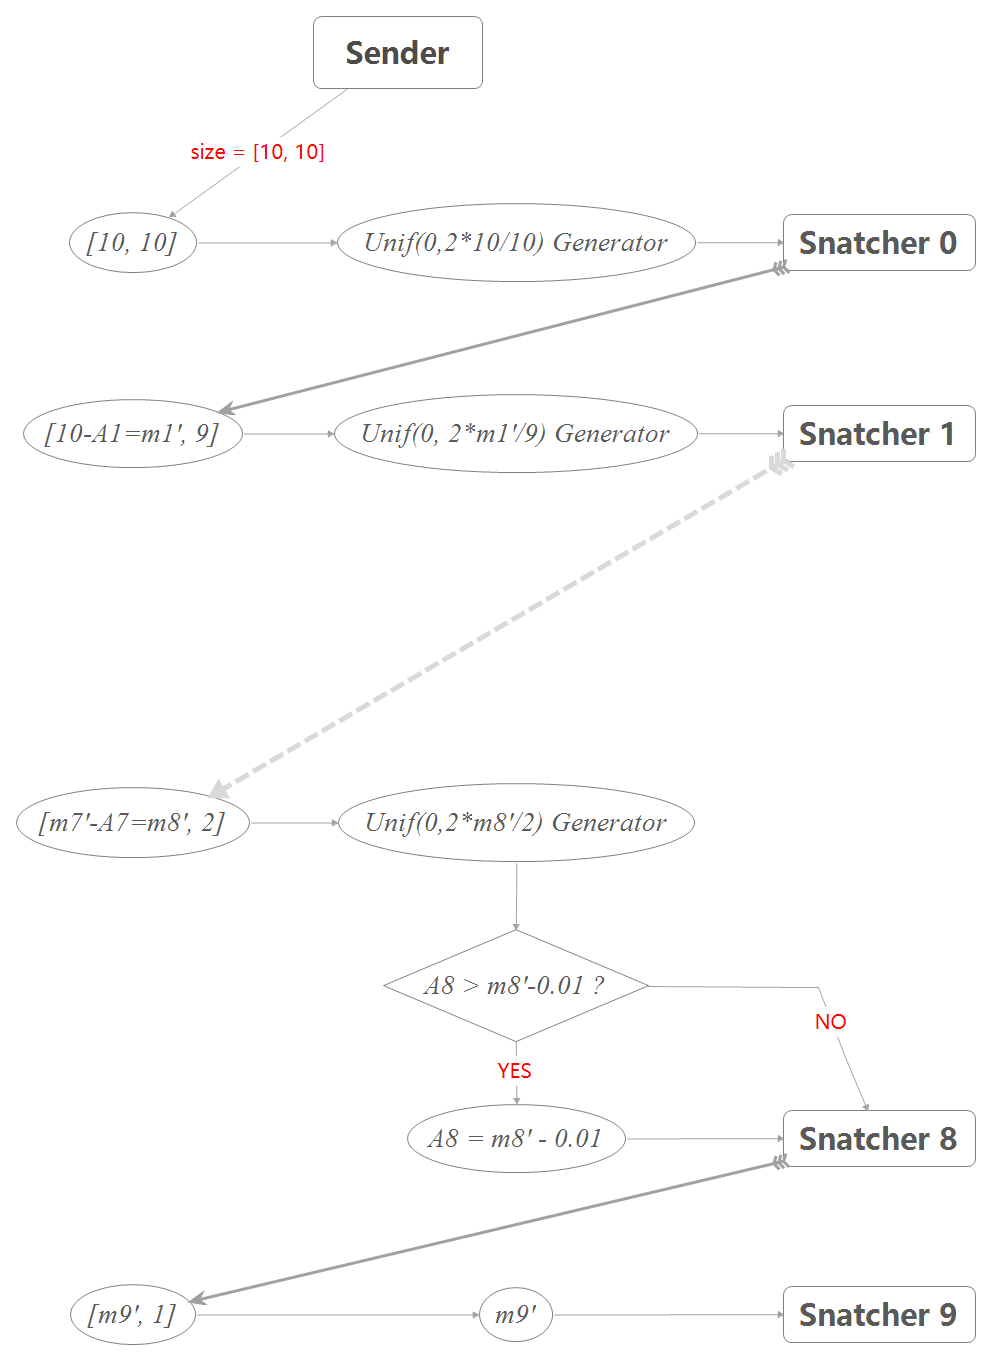
\includegraphics[scale=0.16]{model2.png}
\end{frame}

\begin{frame}{Dynamic-Updating Model}
	\textbf{Mathematical Verifications}:
	\begin{itemize}
		\item Expectation of $A_i$: For the first position, $A_0 \sim$ Unif($0, 2\frac{m}{n}$),
			\[
				E(A_0) = \frac{0 + 2 \times \frac{m}{n}}{2} = \frac{0 + 2 \times \frac{10}{10}}{2} = 1
			\]
			Conditioning on the first position, $A_1|A_0 = a \sim$ Unif($0, 2\frac{m-a}{n-1}$). So according to Adam's Law, for the position 1, we have
			\[
				E(A_1) &= E(E(A_1|A_0)) \\
					&= E(\frac{10 - A_0}{9}) \\
					&= \frac{10 - E(A_0)}{9} \\
					&= 1
			\]
			and similar for the rest positions.
	\end{itemize}
\end{frame}

\begin{frame}{Dynamic-Updating Model}
	\textbf{Mathematical Verifications}:
	\begin{itemize}
		\item The variance of $A_0$ is
			\[
				Var(A_0) = \frac{(2-0)^2}{12} = \frac{1}{3}
			\]
			and according to Eve's Law, variance of $A_1$ at position 1 will be
			\[
				Var(A_1) &= E(Var(A_1|A_0)) + Var(E(A_1|A_0)) \\
					&= E(\frac{(2 \frac{10 - A_0}{9} - 0)^2}{12}) + Var(\frac{10 - A_0}{9}) \\
					&= \frac{247}{9^3} \approx 0.339 > \frac{1}{3} = Var(A_0)
			\]
			which agrees with the increasing variance in insight 2).
	\end{itemize}
\end{frame}

\begin{frame}{Dynamic-Updating Model}
	\begin{itemize}
		\item Also, as the result of extra adjusting at position 8, $A_8$ and $A_9$ suffers more uncertainty than previous positions, which perfectly answers the jump of variance at position 8.
		\item The truncated Normal distribution at latter positions is also a natural consequence under this model. Detailed proof will be omitted.
	\end{itemize}
\end{frame}

\section{Simulations and Testing}

\begin{frame}{Simulation and Testing}
	\ \ Simulation programs of both Static-Uniform model and Dynamic-Updating model are accomplished using \textit{Python} language. In order to conduct hypotheses testing, both programs are run with the same size of red envelope $[10, 10]$ and the same number of samples $202$. After acquiring the simulation results, the following three targets are evaluated and compared to the original data:
	\begin{itemize}
		\item \textbf{Uniformity of Mean}
		\item \textbf{Regression Curve of Variance}
		\item \textbf{Probability Distribution at Positions}
	\end{itemize}
\end{frame}

\begin{frame}{Uniformity of Mean}
	\ \ The mean values of amount of money $A_0, A_1, \dots , A_9$ from original raw data and two simulation models are as follows: \\[10pt]
	\centering
	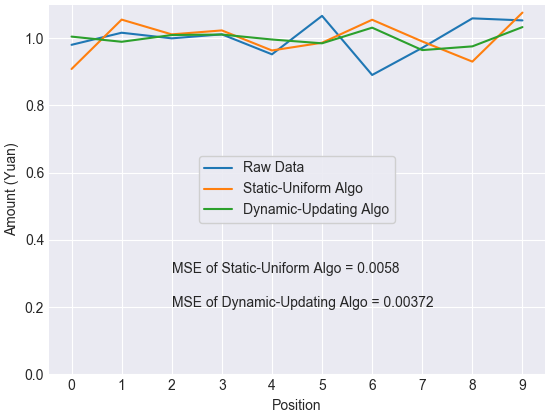
\includegraphics[scale=0.5]{result1.png}
\end{frame}

\begin{frame}{Uniformity of Mean}
	\begin{definition}
		\ \ Denote $\tilde{A_i}$ to be the mean values of raw data, and $\hat{A_i}$ to be the mean values of simulated data, for $i \in \{0, 1, \dots ,9\}$. Mean square error (MSE) of simulation results compared to raw data is defined as
		\[
			MSE = \frac{1}{10} \sum_{j=0}^9 (\hat{A_j} - \tilde{A_j})^2
		\]
		which represents the deviation of mean values from raw data.
	\end{definition}
\end{frame}

\begin{frame}{Uniformity of Mean}
	\textbf{Comparison}:
	\begin{itemize}
		\item $MSE$ of Dynamic-Updating model $\approx 0.00372$
		\item $MSE$ of Static-Uniform model $\approx 0.00580$.
	\end{itemize}
	\vspace{8pt}
	This reveals that the \uline{Dynamic-Updating model generally performs better than Static-Uniform model on approximating mean values}.
\end{frame}

\begin{frame}{Variance Regression}
	\ \ The variance of $A_0, A_1, \dots , A_9$ are sampled and estimated using an order-$2$ regression. The regression plot in shown below: \\[10pt]
	\centering
	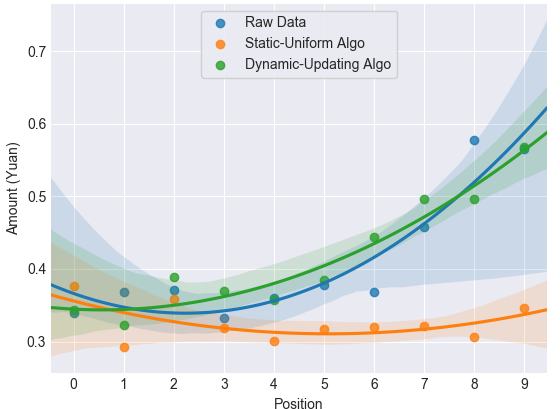
\includegraphics[scale=0.5]{result2.png}
\end{frame}

\begin{frame}{Variance Regression}
	\textbf{Comparison}: \\
	\ \ It can be observed that the output of Dynamic-Updating model follows a perfect regression curve, meanwhile the Static-Uniform model does not reproduce the increasing and jumping variance. Therefore, \uline{Dynamic-Updating model performs much better than Static-Uniform model on approximating the fluctuation of amount of money}.
\end{frame}

\begin{frame}{Distribution at Positions}
	\ \ The distribution of $A_0, A_1, \dots , A_9$ are from original raw data and two simulation models are shown below: \\[10pt]
	\centering
	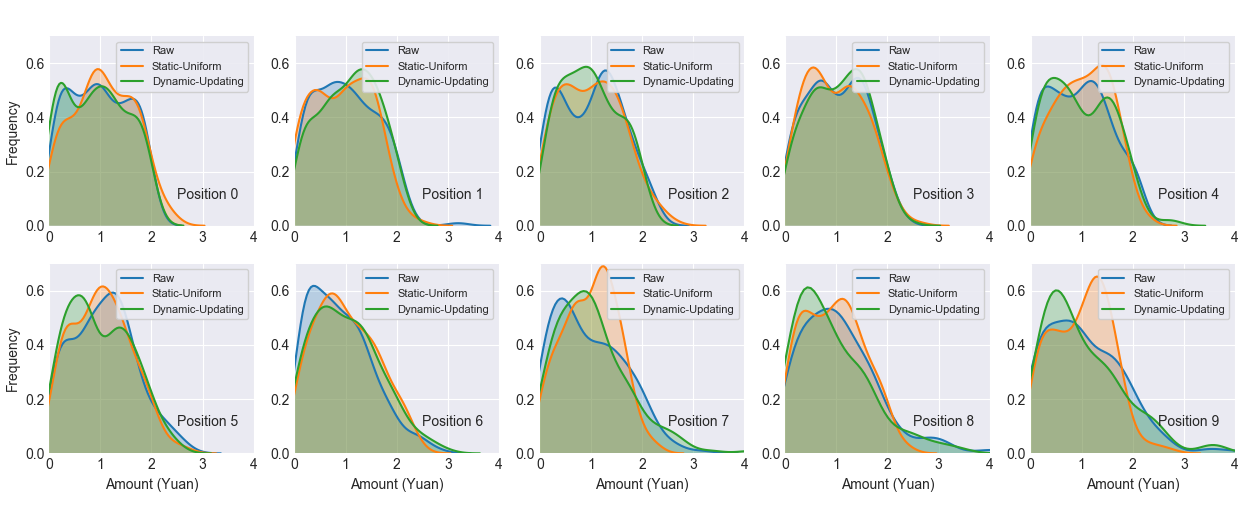
\includegraphics[scale=0.35]{result3.png}
\end{frame}

\begin{frame}{Distribution at Positions}
	\textbf{Comparison}: \\
	\ \ Both Static-Uniform and Dynamic-Updating models perform well in approximating distributions at different positions. However, Static-Uniform algorithm does not reveal the Uniform distribution at earlier positions and the truncated Normal distribution at latter positions as clearly as Dynamic-Updating algorithm. Therefore, \uline{Dynamic-Updating model still performs better than Static-Uniform model on approximating the distribution at each position}.
\end{frame}

\section{Conclusions}

\begin{frame}{Conclusions}
	In summary, the Dynamic-Updating model is a perfect approximation of the Wechat Red Envelope algorithm mechanism.
	\begin{itemize}
		\item It is an online algorithm that generates a uniformly random amount of money ranging from $0.01$ Yuan to twice the mean of rest envelope $2\frac{m_i'}{n-i}$.
		\item It satisfies the uniformity of mean and the increasing variance along the positions, and especially answers the jump of variance at the penultimate position.
	\end{itemize}
\end{frame}

\begin{frame}{Acknowledgement}
	\begin{enumerate}
		\item During this project, I collaborated and discussed with classmates Xinyu Zhang, Ruoyu Wang, Zikun Xiao and Haoyi Zhu.
		\item I also adopted part of contents from Zhihu to Section III about the idea of dynamic algorithm mechanism.
		\item Original red envelope data is collected in two chat groups on WeChat with in total 36 student members. I appreciate Ruoyu Wang and Yuyan Zhou for helping to collect the raw data.
	\end{enumerate}
\end{frame}

\begin{frame}{References}
	\scriptsize
	\bibliographystyle{IEEEtran}
	\bibliography{Reference}
\end{frame}

\end{document}
